\documentclass[border=0.65cm,tikz]{standalone}
\usepackage[utf8]{vietnam}
\usepackage{xcolor}
\definecolor{dnvang}{HTML}{D8A25E}
\definecolor{dnxanh}{HTML}{229799}
\definecolor{dnxanhdam}{HTML}{0D7C66}
\definecolor{dndo}{HTML}{BB2649}
\def\mycolor{dnvang}
\def\mauphu{dnxanh}
\def\maudam{dnxanhdam}
\def\maunhan{dndo}
\usepackage{tikz}
\usepackage{tikz-3dplot}
\usepackage{pgfplots}
\pgfplotsset{compat=1.18}
\usetikzlibrary{angles,quotes,intersections,fit}
\usetikzlibrary{calc,fadings,shadows,shadows.blur,shapes,shapes.geometric,positioning,backgrounds,decorations.pathmorphing,decorations,matrix}
\usetikzlibrary{decorations.pathmorphing}
\begin{document}
	\newcommand{\khungion}[2][+]{%
		\tikz[baseline=(ND).base]{
			\node[inner sep=0pt,outer sep=3pt,align=center](ND){#2};
			\draw[rounded corners=0.5pt,line cap=round,line join=round] ($(ND.north west)+(3pt,0)$)--(ND.north west)--(ND.south west)--($(ND.south west)+(3pt,0)$);
			\draw[rounded corners=0.5pt,line cap=round,line join=round] ($(ND.north east)+(-3pt,0)$)--(ND.north east)coordinate (D)--(ND.south east)--($(ND.south east)+(-3pt,0)$);
			\path(D) node[shift={(45:5pt)}]{\scriptsize\textbf{#1}};
		}
	}
	%%%Xu hướng nhận e của K
	\newcommand{\muiten}[1][\mycolor]{%
		\tikz{
			\fill[#1](0,0)--++(-90:6pt) coordinate (A)
			--++(-1.8cm,0)--++(-90:12pt)--++(0:1.8cm)coordinate (B)
			--++(-90:6pt)--($(A)!0.5!(B)+(0.5cm,0)$)--cycle;
		}
	}
	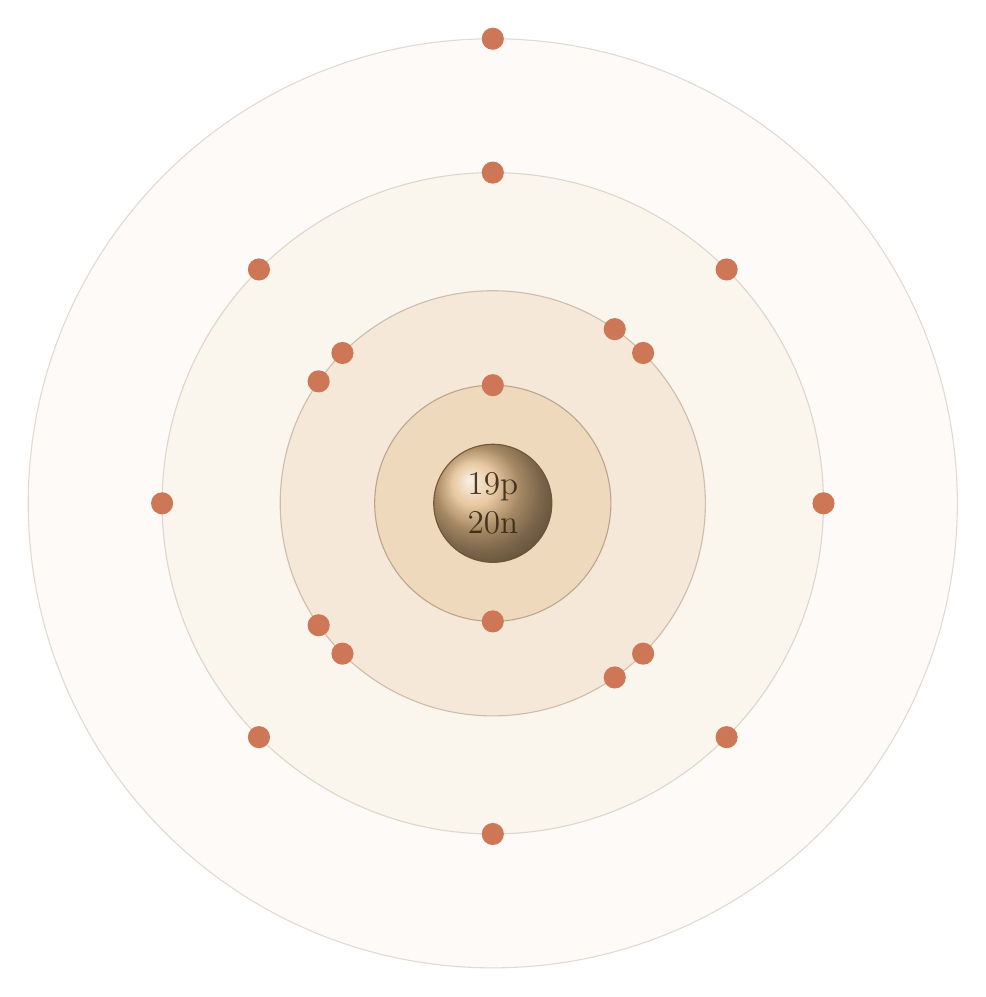
\begin{tikzpicture}[declare function={%
			r1=0.75cm;
			r2=1.5cm;
			r2h=r2+4pt;
			r3=2.7cm;r3h=r3+6pt;
			r4=4.2cm;r4h=r4+7pt;
			r5=5.9cm;r5h=r5+8pt;
			d=8cm;
		}
		]%
		\tikzset{
			potasium/.pic={%
				\path[fill=\mycolor!25,opacity =0.2,pic actions] (0,0) circle (r5);
				\path[fill=\mycolor!35,opacity =0.2,pic actions] (0,0) circle (r4);
				\path[fill=\mycolor!55,opacity =0.3,pic actions] (0,0) circle (r3);
				\path[fill=\mycolor!65,opacity =0.4,pic actions] (0,0) circle (r2);
				\path[ball color=\mycolor!80,opacity =0.9,pic actions] (0,0) circle (r1) node[font=\large\fontfamily{qag}\selectfont,text=\mycolor!25!black,text width=1cm,align=center] {\textbf{19p} \\ \textbf{20n}};
				\foreach \g/\r in{90/r2,-90/r2}{%
					\fill (\g:\r) [\maunhan!35!\mycolor] circle (4pt);
				}
				%%
				\foreach \g/\r in{-45/r3,-55/r3,-135/r3,-145/r3,45/r3, 55/r3,135/r3,145/r3}{%
					\fill (\g:\r) [\maunhan!35!\mycolor] circle (4pt);
				}
				%%
				\foreach \i in{1,2,3,4,5,6,7,8}{
					\foreach \g/\r in{{-90+\i*360/8}/r4}{%
						\fill (\g:\r) [\maunhan!35!\mycolor] circle (4pt);
					}
				}
				%%%
				\foreach \g/\r in{90/r5}{%
					\fill (\g:\r) [\maunhan!35!\mycolor] circle (4pt);
				}
			},
			potasiumH/.pic={
				\path[fill=\mycolor!55,opacity =0.3,pic actions] (0,0) circle (r4h);
				\path[fill=\mycolor!55,opacity =0.3,pic actions] (0,0) circle (r3h);
				\path[fill=\mycolor!65,opacity =0.4,pic actions] (0,0) circle (r2h);
				\path[ball color=\mycolor!80,opacity =0.9,pic actions] (0,0) circle (r1) node[font=\large\fontfamily{qag}\selectfont,text=\mycolor!25!black] {$\textbf{+Z}$};
				\foreach \g/\r in{90/r2h,-90/r2h}{%
					\fill (\g:\r) [\maunhan!35!\mycolor] circle (4pt);
				}
				%%
				\foreach \g/\r in{-45/r3h,-55/r3h,-135/r3h,-145/r3h,45/r3h, 55/r3h,135/r3h,145/r3h}{%
				\fill (\g:\r) [\maunhan!35!\mycolor] circle (4pt);
				}
				%%%
				\foreach \i in{1,2,3,4,5,6,7,8}{
					\foreach \g/\r in{{90+\i*360/8}/r4h}{%
						\fill (\g:\r) [\maunhan!35!\mycolor] circle (4pt);
					}
				}
			},
			stylefont/.style={font=\bfseries\LARGE\fontfamily{qag}\selectfont,text=\mycolor!25!black}
		}
		\path (0,0) pic[local bounding box =na,draw=\mycolor!50!black] {potasium};
	\end{tikzpicture}
\end{document}